This section contains the results of the comparison between the CAM and WACCM simulations. 

\subsection{Temperature Targets}
The deviations from the temperature targets in Eq. \ref{eq:Tpsi} were calculated from 2-meter temperature for all simulations. The results are shown in Figure \ref{fig:Tgrad1}. The results from the SSP5-8.5 simulations with CAM and WACCM are near identical for $T_0$, showing comparable variability and arriving at virtually the same final GMST. The results from the gradual SAI simulations are also comparable, both simulations succeeding in maintaining 2020 GMST levels with comparable variability. 

Deviations from $T_1$ and $T_2$ are again comparable in CAM and WACCM. The SSP5-8.5 simulation in CAM arrives at a deviation from $T_1$ about 25\% lower than in WACCM. Trendline analysis (not shown) confirms that the increase in $\Delta T_1$ in CAM is about 30\% lower than in WACCM. The trend in $Delta T_2$ is about 20\% lower in CAM than in WACCM. Though significant, qualitatively the behaviour of CAM is very similar to that of WACCM and the difference can be attributed to individual model response. The gradual SAI simulation in CAM is  comparable to WACCM, maintaining $T_1$ and $T_2$ with similar variability and no significant trend in either model.

% [0.00339544 0.02208369]
% 0.00025031442996526897 0.011112946002398446
% [ 0.00486383 -0.00078264]
% 0.00019685314966332964 0.00885292479449391
% [0.00391574 0.00179368]
% 0.00019010752177689276 0.008440003545960452
% [ 0.00502745 -0.0091592 ]
% 0.0001932863742419903 0.00869251635848846

% [-0.00067792  0.05548463]
% 0.0002825888875922955 0.012929792774639662
% [-0.00226457  0.0537639 ]
% 0.0012696237327225347 0.05919769566467151
% [-0.00104812  0.06099048]
% 0.00021350422234038088 0.009768838974727728
% [-0.00050996  0.01638082]
% 0.00024406425653920928 0.011379782266976644


\begin{figure}[H]
	\centering
	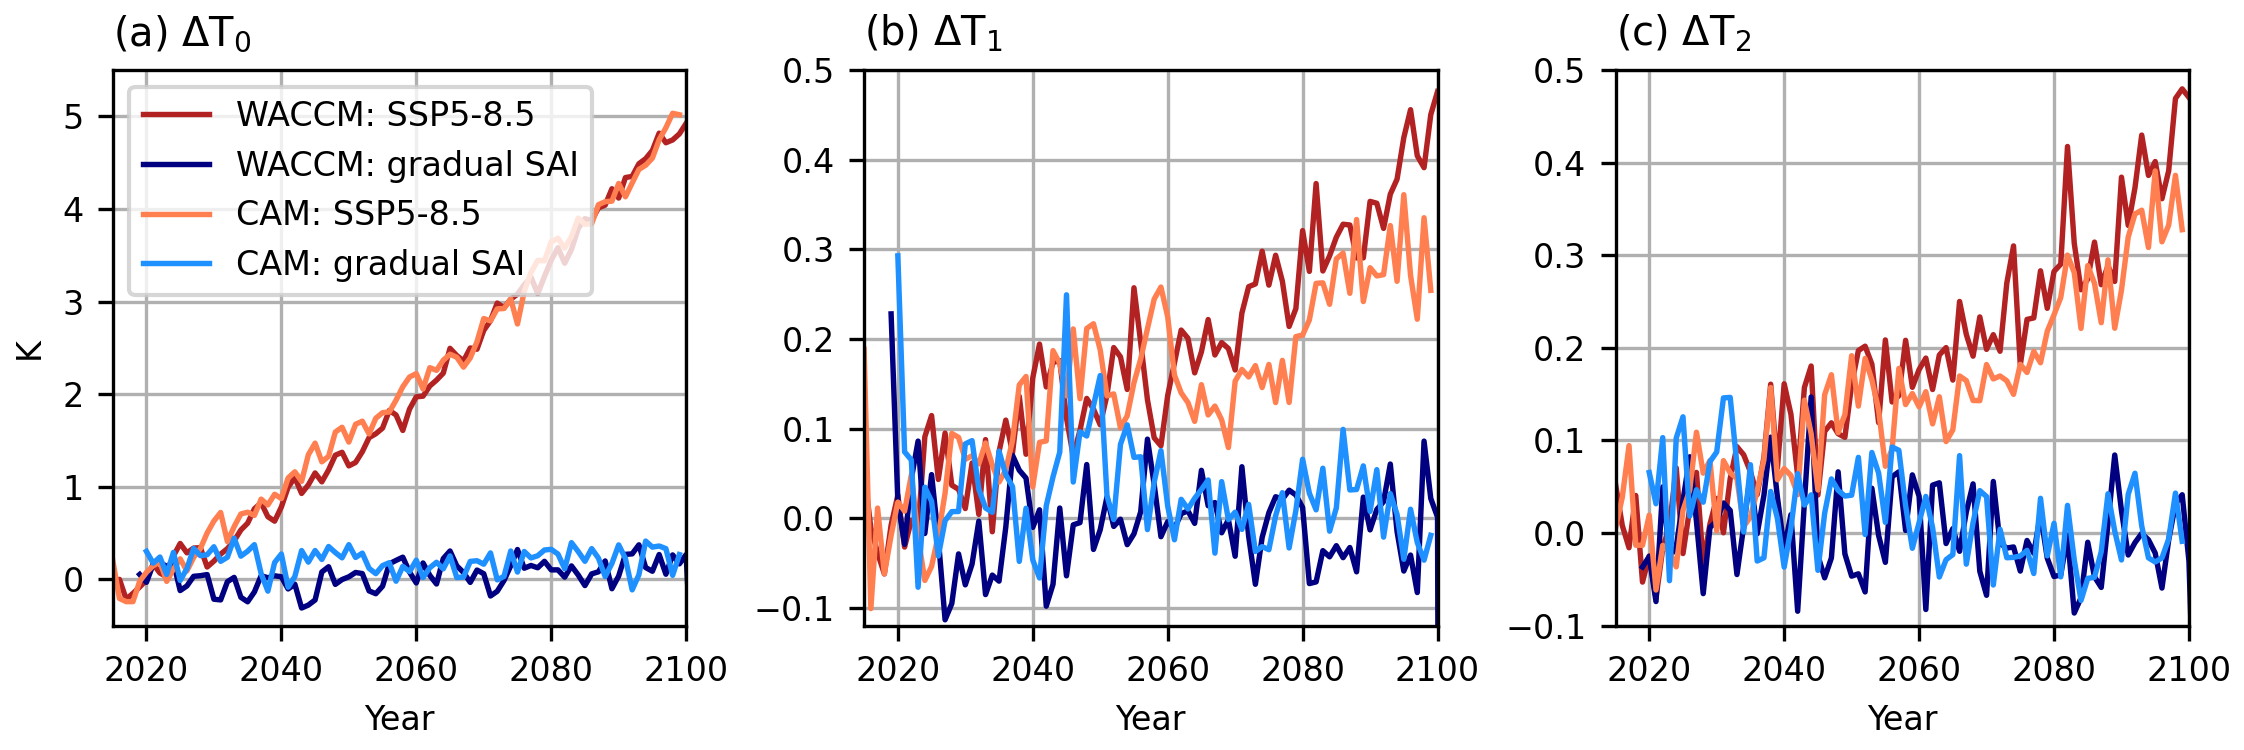
\includegraphics[width=0.95\linewidth]{images/Tgrad_v.png}
	\caption{Deviations from temperature targets $T_0$, $T_1$, $T_2$ as compared to 2016-2025 mean, for the SSP5-8.5 and gradual SAI scenarios in CAM and WACCM.}
	\label{fig:Tgrad1}
\end{figure}


\subsection{2-meter Temperature and Precipitation in CAM}
Figure \ref{fig:CAM_scens} shows the Reference 2-meter temperature and precipitation, their anomalies for Control compared to the Reference and their anomalies for SAI 2020 compared to Control. In Figure \ref{fig:CAM_scens}(b) the Control period shows expected warming patterns, with the land area warming more than the sea and the poles warming more relatively due to polar amplification. Anomalous warming off the coast of Antarctica and in the Arctic Ocean indicates a retreat of sea-ice at both poles. The anomalous warming over the eastern Pacific ocean resembles the spatial sea surface temperature pattern of El Ni\~no. The slight cooling over the northern Atlantic ocean resembles a North Atlantic warming hole, generally attributed to changes in ocean heat transport and weakening of the Atlantic meridional overturning circulation (AMOC) but also atmospheric circulation changes due to anthropogenic forcing \parencite{menary2018anatomy,he2022}. 

The SAI 2020 anomaly compared to the Control, shown in Figure \ref{fig:CAM_scens}(c), shows that SAI is able to compensate for most of the warming in Control. The land area is cooled more than the sea, as are the poles. Sea-ice retreat is largely prevented in both the Arctic and the Antarctic. The anomalous warming over the eastern Pacific ocean is not prevented, as is the North Atlantic warming hole. 

The precipitation anomaly in Control, shown in Figure \ref{fig:CAM_scens}(e), shows a general increase in precipitation. Most significant drying can be attributed to a shift in the intertropical convergence zone (ITCZ), with a southward shift over the Atlantic and eastern Pacific Ocean, expected patterns under increased anthropogenic forcing \parencite{mamalakis2021zonally}. The shift over the eastern Pacific Ocean is possibly related to the El Ni\~no-like warming observed in Fig. \ref{fig:CAM_scens}(b). No significant shift or other change in ITCZ is observed over the Indian and western Pacific Ocean.

In Figure \ref{fig:CAM_scens}(f) the precipitation anomaly of SAI 2020 compared to Control shows opposite trends, apparently preventing most increase in precipitation. The southward shift of the ITCZ is mostly prevented, though not entirely over the eastern Pacific.

\begin{figure}[H]
	\centering
	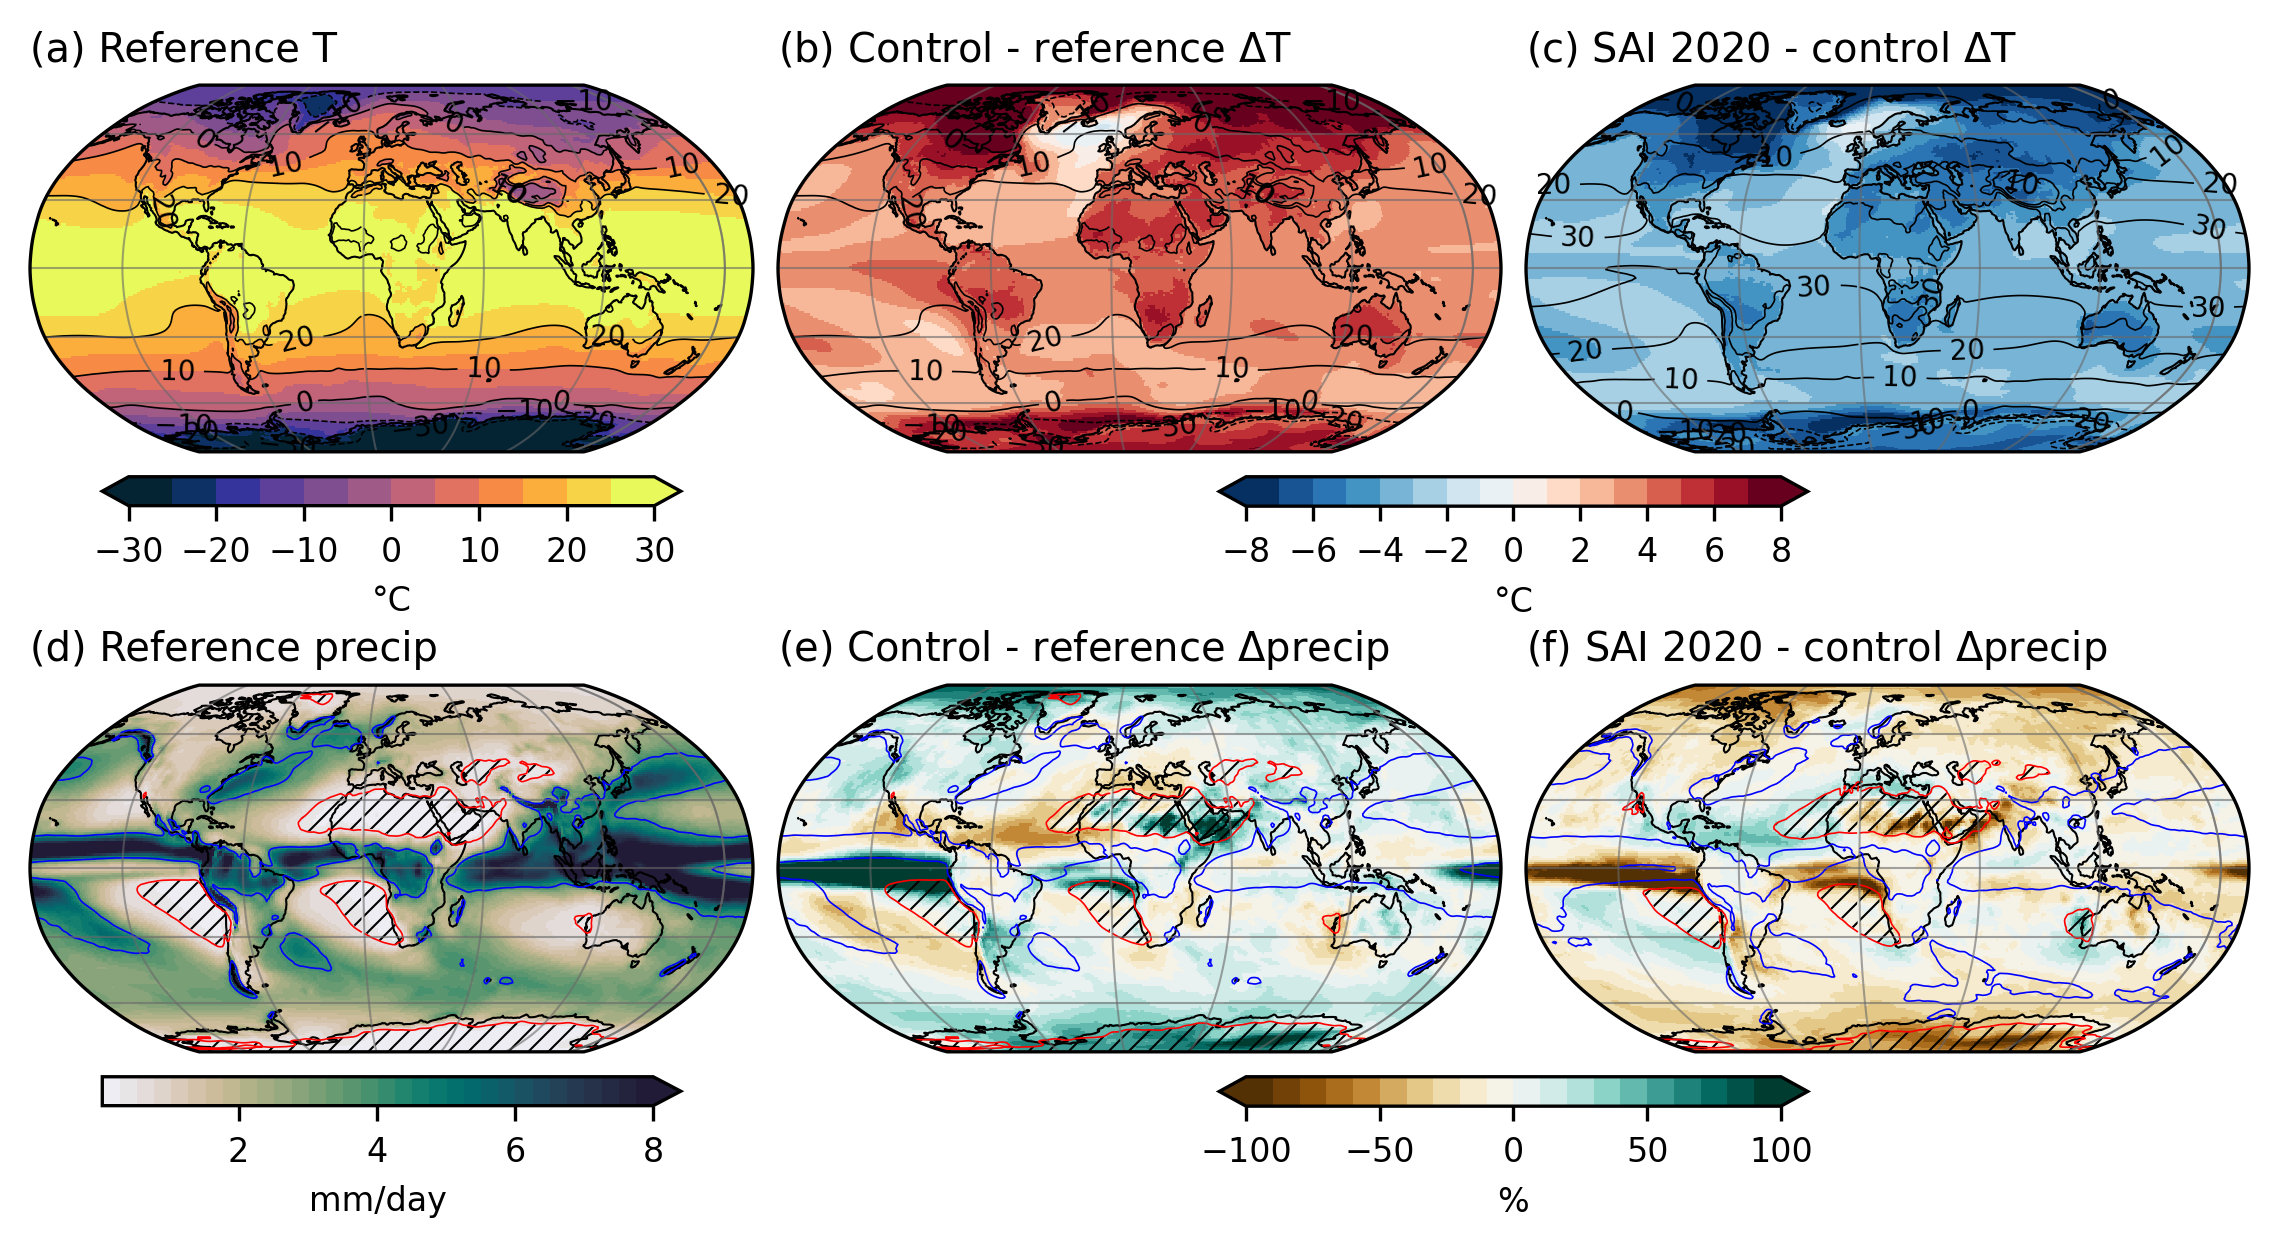
\includegraphics[width=0.95\linewidth]{images/CAM_scens.png}
	\caption{CAM model results; (a): Reference annual mean 2-meter temperature with contours in 10°C intervals; (b): Annual mean 2-meter temperature anomaly for Control compared to Reference, Reference shown in black contours in 10°C intervals; (c): Annual mean 2-meter temperature anomaly for SAI 2020 compared to Control, contours as in (b) but for Control; (d): Reference annual mean precipitation in mm/day, 4 mm/day shown in blue contours, $<0.3$mm/day shown in red contours with hatching; (e) Annual mean precipitation anomaly for Control compared to Reference, contours as in (d); (f): Annual mean precipitation anomaly for SAI 2020 compared to Control, contours as in (d) but for Control.}
	\label{fig:CAM_scens}
\end{figure}


\subsection{SAI 2020 2-meter Temperature Anomalies in CAM and WACCM}
The annual and seasonal mean 2-meter temperature anomalies of SAI 2020 compared to the Reference for CAM and WACCM are shown in Figure \ref{fig:TREFHT_20ref}. Figure \ref{fig:TREFHT_20ref}(c) shows the difference between (a) and (b), i.e. the inter-model difference corrected for their difference in SAI 2020. Figures \ref{fig:TREFHT_20ref}(f) and (i) show the annual and seasonal zonal mean anomalies for CAM and WACCM respectively. 

The annual mean anomalies in Figures \ref{fig:TREFHT_20ref}(a) and (b) show a generally similar pattern of warming over the tropics, cooling over the subtropics and warming over the poles. The Arctic warms more in CAM than it does in WACCM, at most 3°C. Both models show significant cooling over the nothern Atlantic Ocean, again resembling the North Atlantic warming hole seen in Figure \ref{fig:CAM_scens}, CAM more so than WACCM. The El Ni\~no pattern in the eastern Atlantic is visible in both models, though more pronounced in CAM. 

Figure \ref{fig:TREFHT_20ref}(c) confirms the patterns described above. The figure also highlights the difference in response over North America and off the coast of Antarctica between 0° and 30°E, where CAM slightly cools and WACCM slightly warms, leading to a significant difference.

In Figures \ref{fig:TREFHT_20ref}(d) and (e), the seasonal response of CAM is shown. Comparison between the two seasons and the annual mean shows that most warming at the poles occurs during their respective winter. This is further confirmed by the zonal mean anomaly in Figure \ref{fig:TREFHT_20ref}(f). The El Ni\~no-like pattern in the eastern Pacific Ocean is stronger in magnitude in JJA, though more expansive in DJF, though neither anomaly shows up in the zonal mean anomaly figure. 

The same patterns as in the annual mean are visible in Figures \ref{fig:TREFHT_20ref}(g) and (h), with the Antarctic as a whole warming in the Southern Hemisphere winter and the Barentsz sea in the Arctic warming significantly in the Northern Hemisphere winter. This pattern is confirmed by Figure \ref{fig:TREFHT_20ref}(i). 

The differing response between the two models in the Arctic and Antarctic temperatures is possibly a result of model-specific sensitivity to cloud feedbacks, which are known to be one the greatest sources of uncertainty in climate modeling \parencite{schneider2017climate}.



\begin{figure}[H]
	\centering
	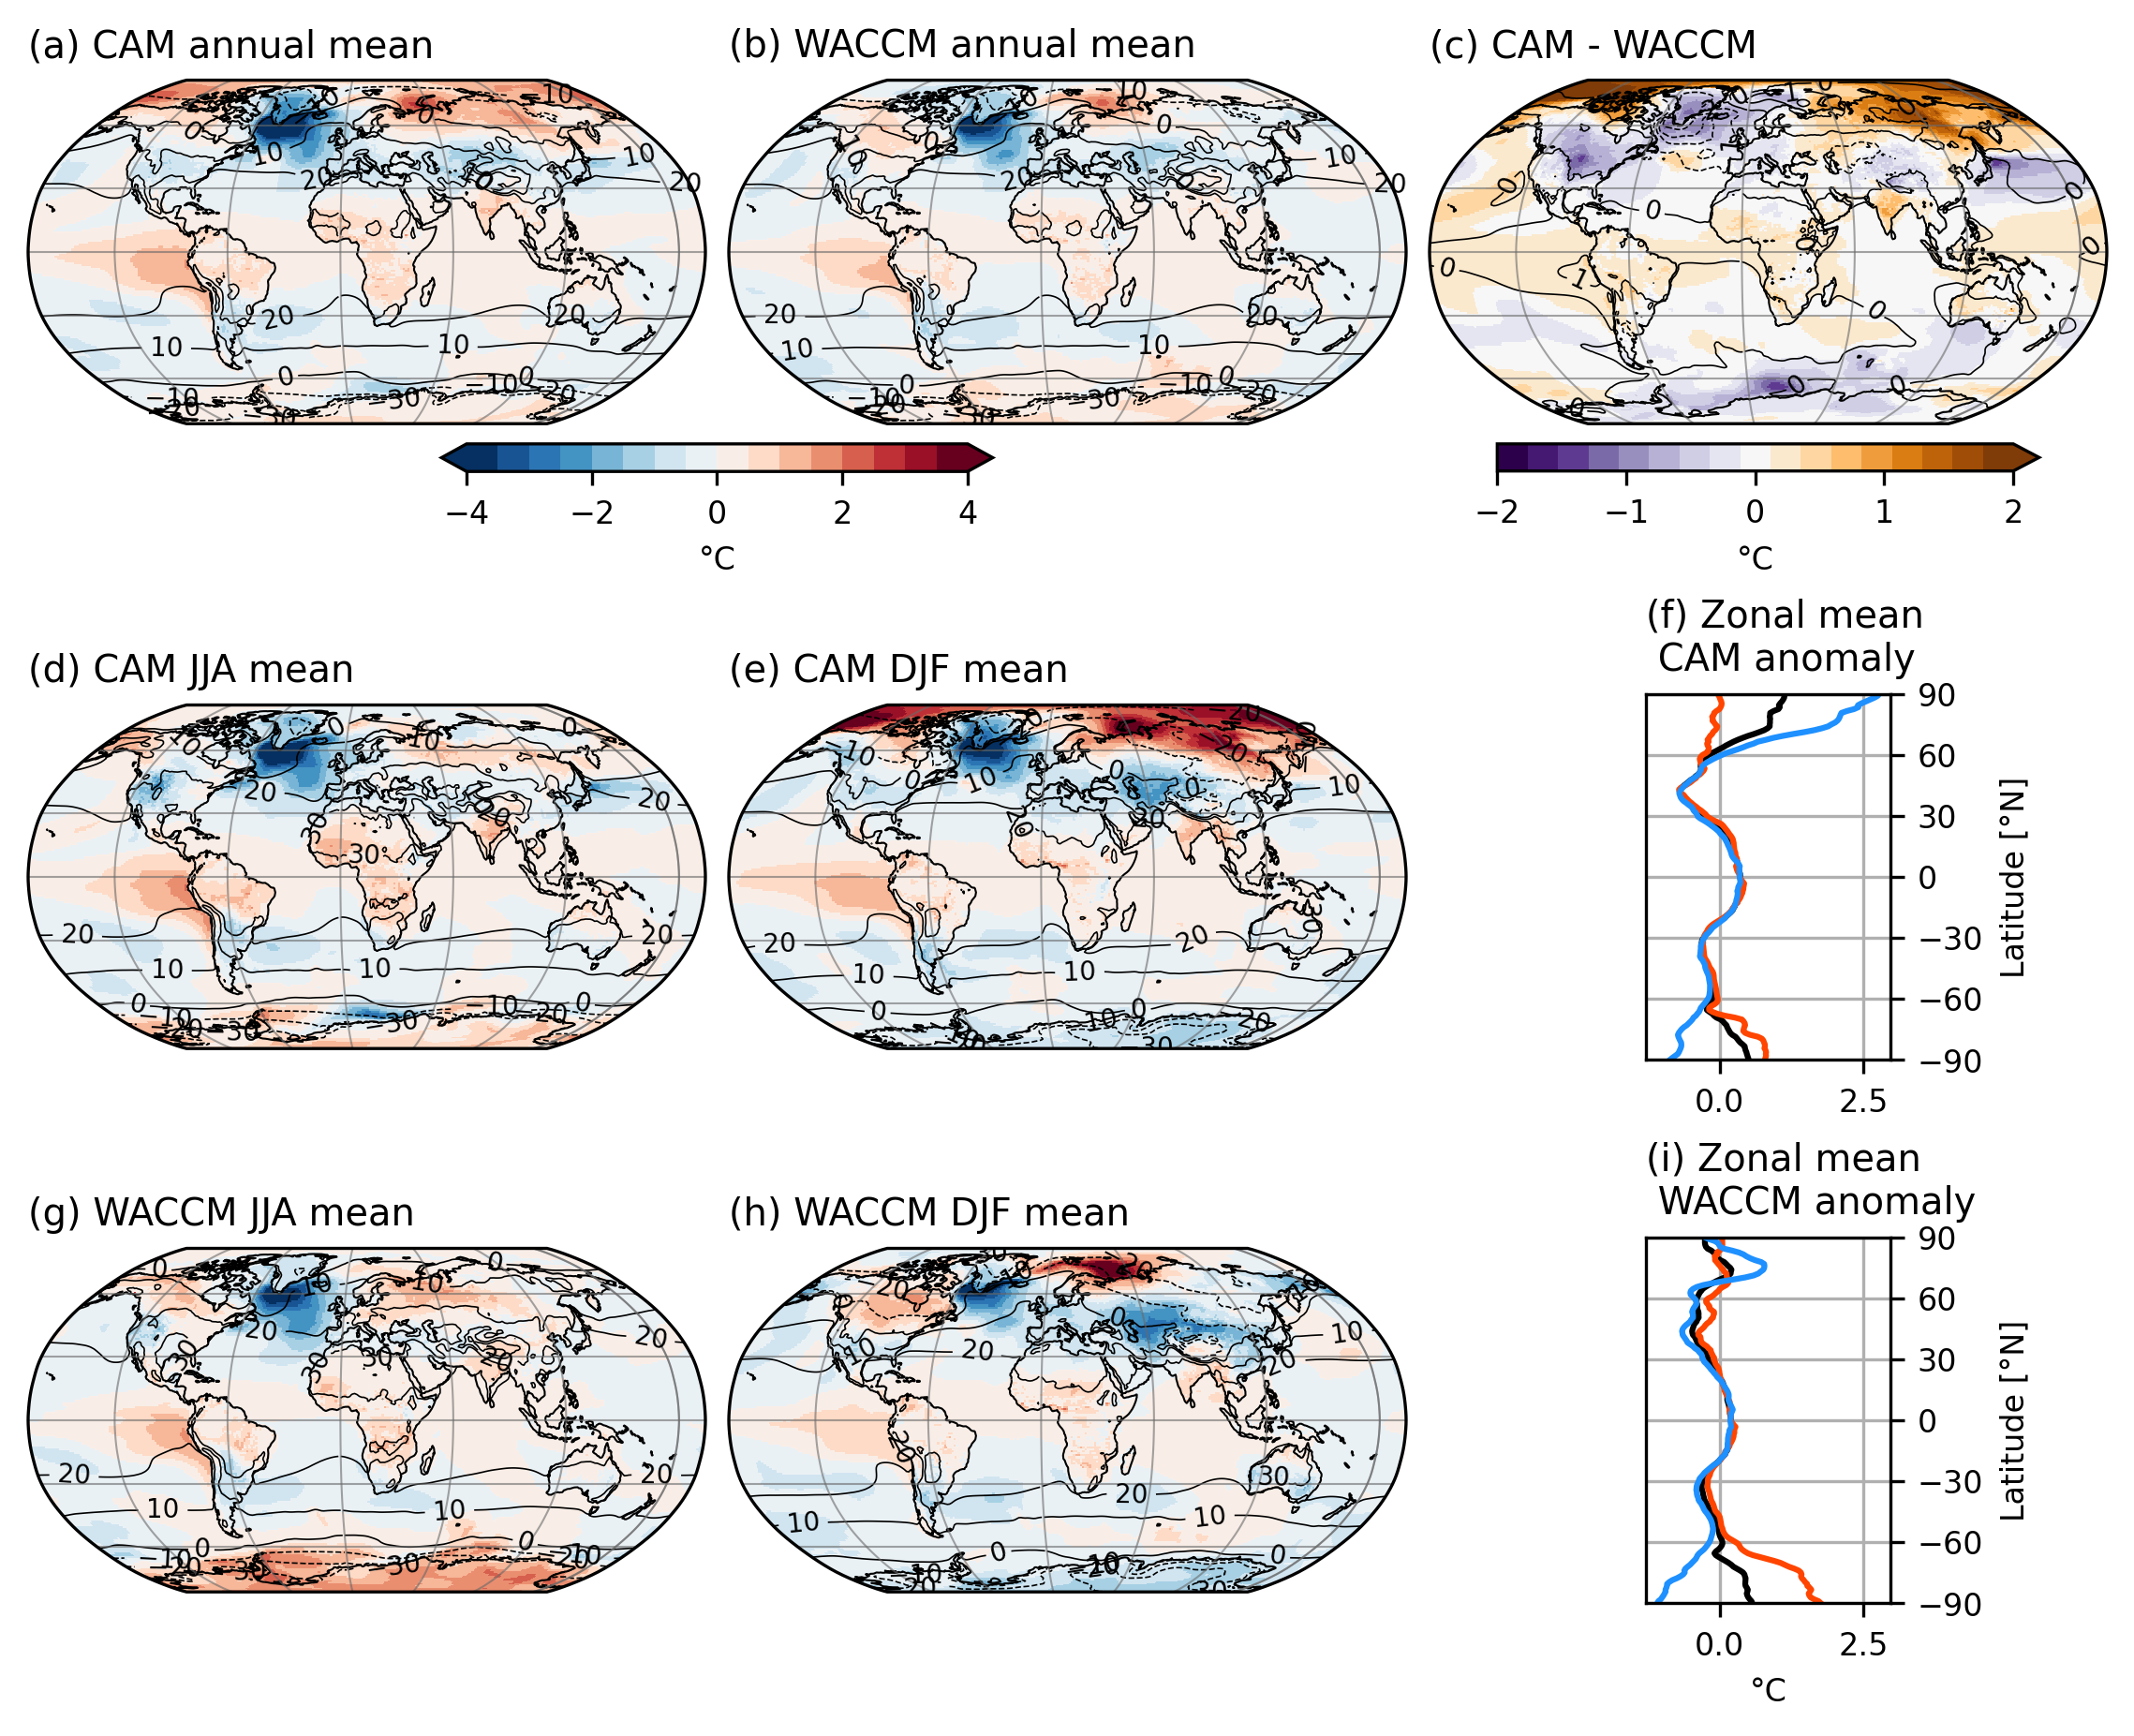
\includegraphics[width=0.95\linewidth]{images/TREFHT_20ref.png}
	\caption{(a,b): Annual mean 2-meter temperature anomalies of SAI 2020 compared to Reference in (a) CAM and (b) WACCM. Reference mean temperature shown in black contours in 10°C intervals; (c): Difference between CAM and WACCM temperature anomalies. WACCM anomaly shown in black contours in 1°C intervals; (d,e): CAM 2-meter temperature anomalies as in (a,b) for (d) JJA and (e) DJF; (f): CAM zonal average 2-meter temperature anomaly as in (a,d,e), annual mean anomaly in black, JJA anomaly in red, DJF anomaly in blue; (g,h,i): analogous to (d,e,f) for WACCM.}
	\label{fig:TREFHT_20ref}
\end{figure}


\subsection{SAI 2020 Precipitation Anomalies in CAM and WACCM}
The annual and seasonal mean precipitation anomalies of SAI 2020 compared to Reference for CAM and WACCM are shown in Figure \ref{fig:PRECT_20ref}. Figure \ref{fig:PRECT_20ref}(c) shows the difference between (a) and (b) as above in Figure \ref{fig:TREFHT_20ref}, note that this difference is given in percentage points. Figures \ref{fig:PRECT_20ref}(f) and (i) show the annual and seasonal zonal mean anomalies for CAM and WACCM respectively.

The annual mean anomalies in Figures \ref{fig:PRECT_20ref}(a) and (b) show a similar pattern overall, with a small decrease in precipitation over most of the globe and larger increase in drier areas and the tropical oceans. CAM shows a much larger precipitation increase over the eastern Pacific Ocean, with a southward shift of the ITCZ. This shift is possibly correlated with the observed anomalous warming in the region (see Figure\ref{fig:TREFHT_20ref}). Contrastingly WACCM shows a larger increase than CAM over dry areas like the Arabian Peninsula.

The same patterns are observed in the seasonal precipitation anomalies in Figures \ref{fig:PRECT_20ref}(d), (e), (g) and (h), with the exception of southern Brazil, where CAM shows a larger increase than WACCM in the JJA mean. The zonal mean anomalies in Figures \ref{fig:PRECT_20ref}(f) and (i) confirm the observed trends further, showing that precipitation in the ITCZ increases twice as much in CAM compared to WACCM, as does precipitation in the Arctic. The Antarctic shows the opposite trend, getting more wet in WACCM than in CAM.


\begin{figure}[H]
	\centering
	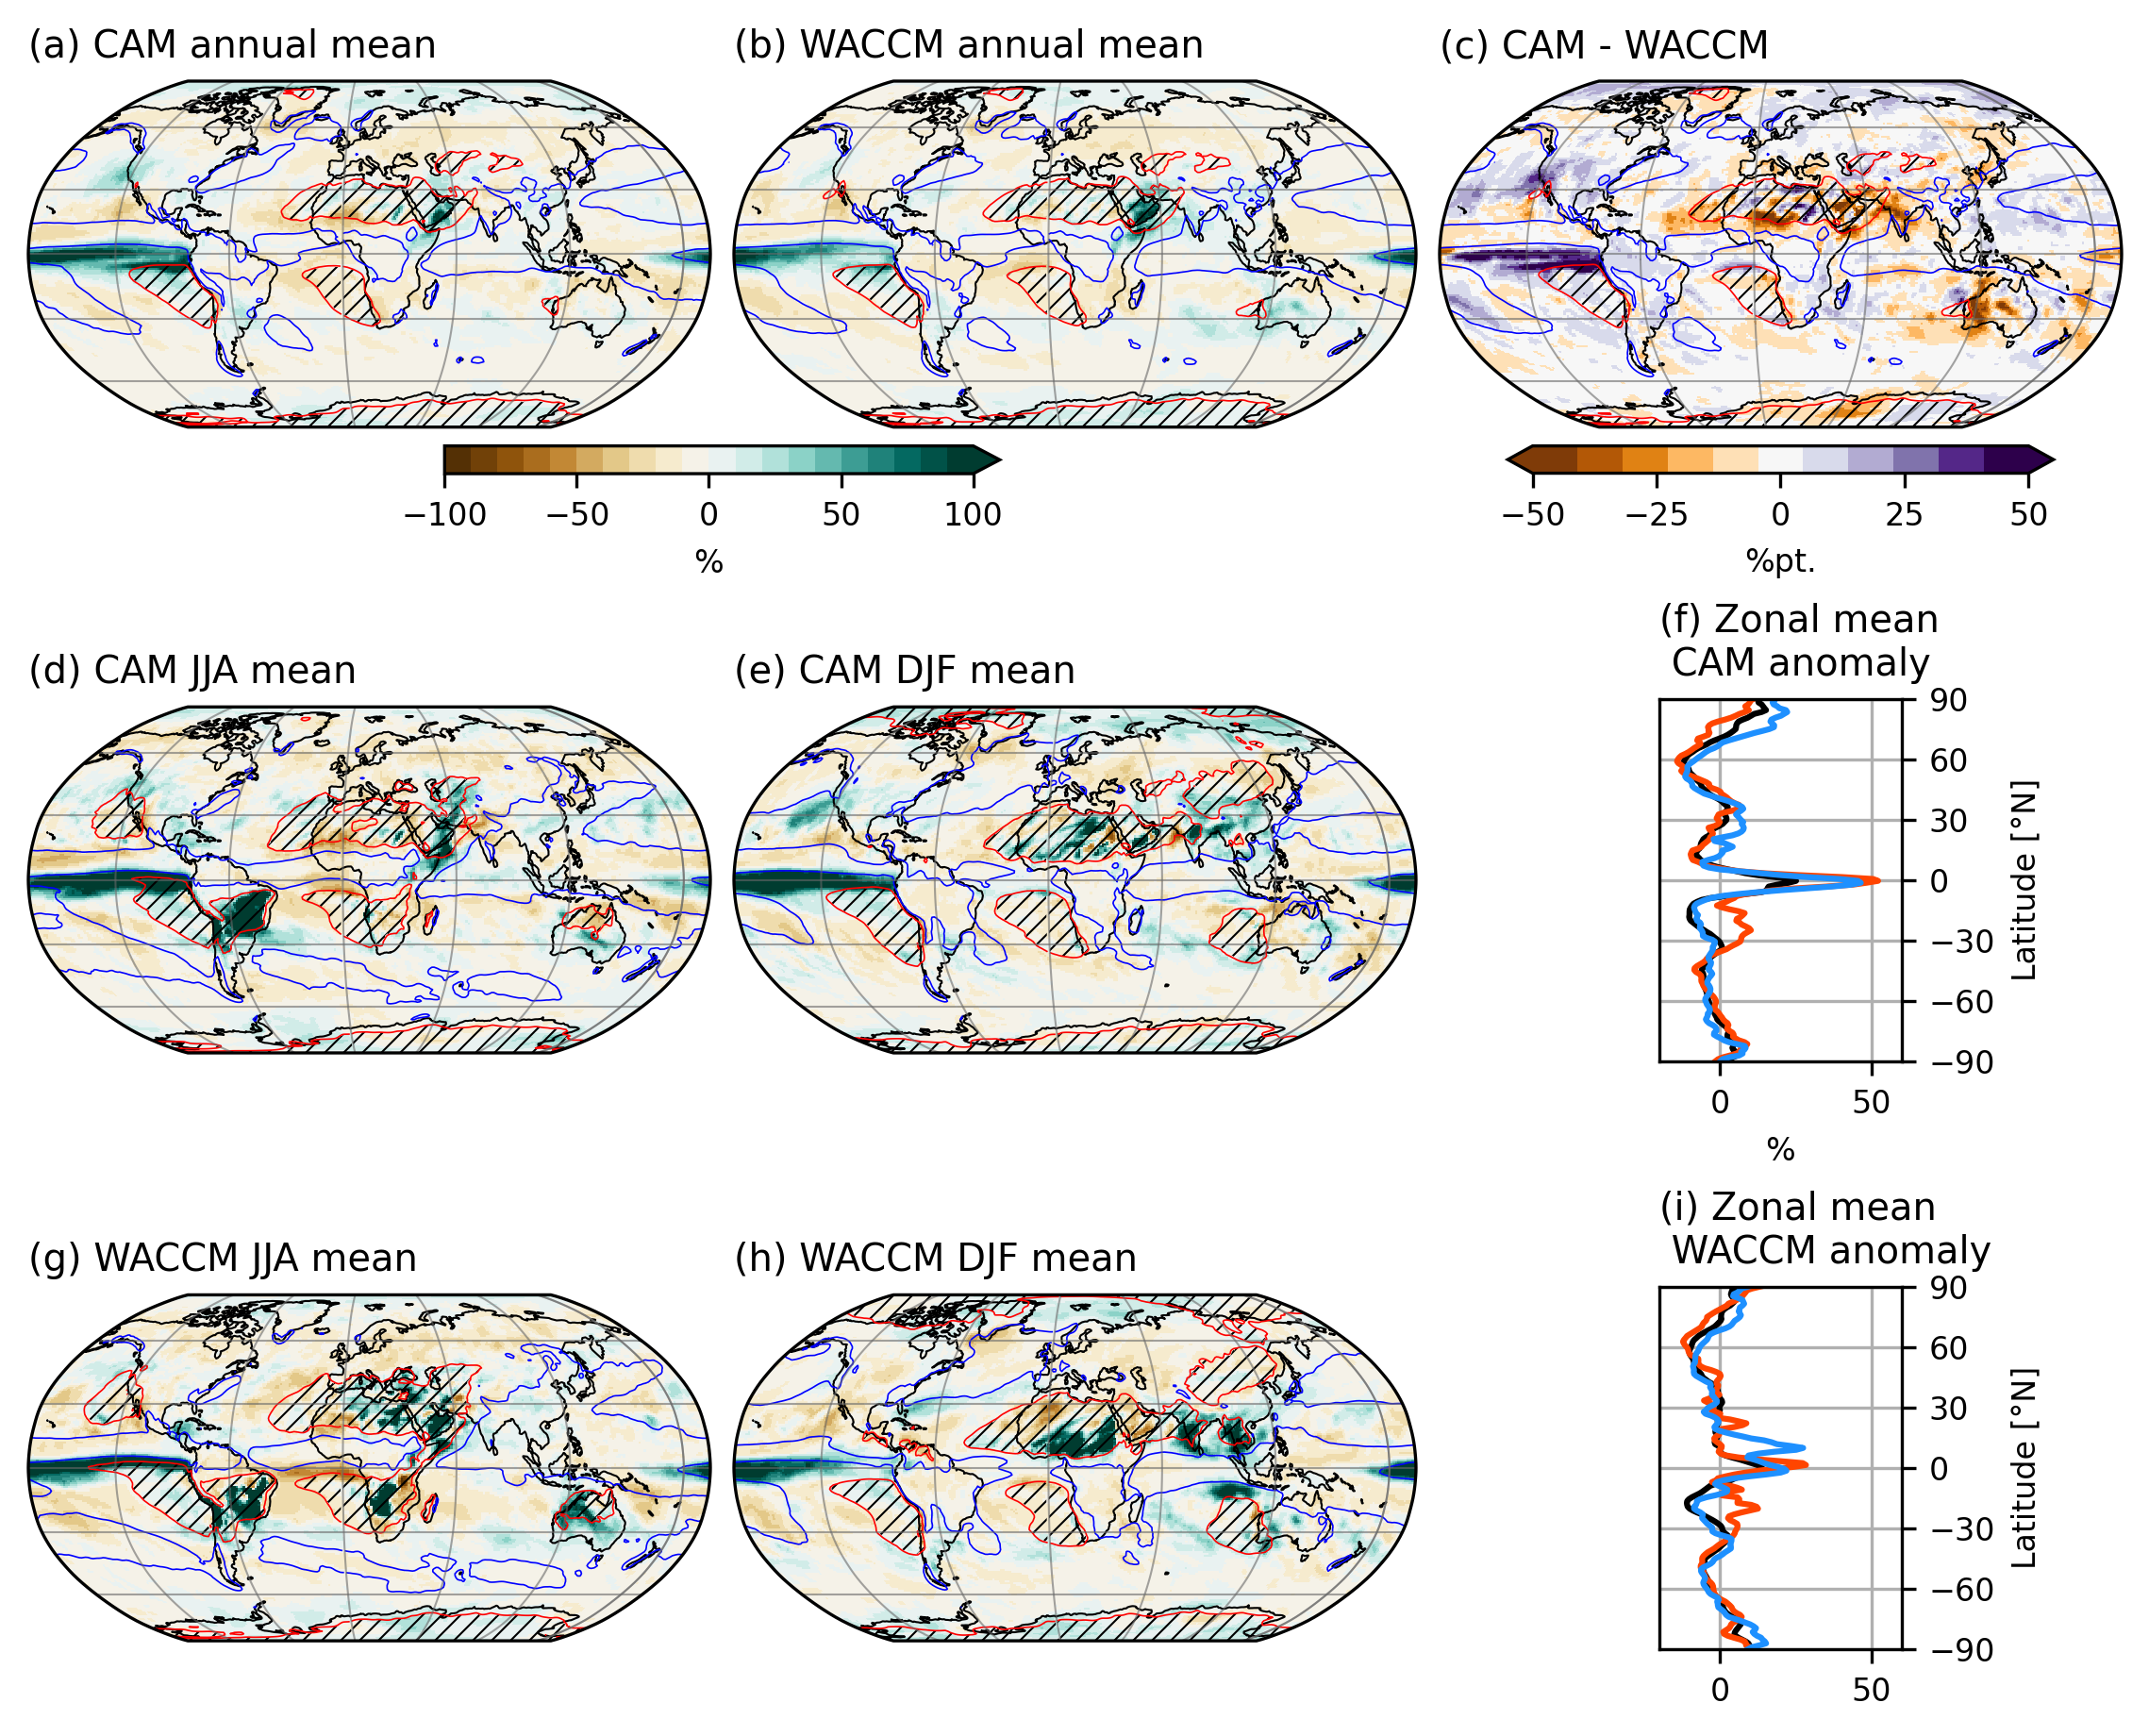
\includegraphics[width=0.95\linewidth]{images/PRECT_20ref.png}
	\caption{(a,b): Annual mean precipitation anomalies of SAI 2020 compared to Reference in (a) CAM and (b) WACCM. Reference mean precipitation shown, 4 mm/day in blue, $<0.3$mm/day in red with hatching; (c): Difference between CAM and WACCM precipitation anomalies. WACCM Control mean precipitation as in (b); (d,e): CAM anomalies as in (a,b) for (d) JJA and (e) DJF; (f): CAM zonal average precipitation anomaly as in,  annual mean anomaly in black, JJA anomaly in red, DJF anomaly in blue; (g,h,i): analogous to (d,e,f) for WACCM.}
	\label{fig:PRECT_20ref}
\end{figure}


\subsection{SAI 2020 Potential Temperature and Zonal Wind Anomalies in CAM and WACCM}\label{th_U_pt1}
The zonal mean potential temperature $\theta$ anomaly and the zonal mean zonal wind anomaly for CAM and WACCM are shown in Figure \ref{fig:th_U_full}, for both the annual and seasonal means. 
In Figures \ref{fig:th_U_full}(a)-(f) the potential temperature anomaly shows significant warming in the stratosphere, in a pattern reminiscent of the aerosol field from Figure \ref{fig:strataero}. Concentrated around 15°N/S and 30°N/S, around 50 hPa in the stratosphere, and around the equator. The warming extends to the poles only in the summer hemisphere, due to the poles receving little to no radiation during the polar night in their respective winter. 

The cooling observed in CAM over the Arctic in winter is not observed in WACCM at the same magnitude, any cooling extends to about the same altitude, but is not as severe as it is in CAM. CAM also shows more cooling than WACCM in the Antarctic winter, though the difference is not as stark as in the Arctic. The cooling effect of greenhouse gases in the upper stratosphere is visible in CAM and WACCM in the annual and seasonal means. There is no significant potential temperature change observed below about 300 hPa. 

The zonal mean zonal wind anomaly in Figures \ref{fig:th_U_full}(g)-(l) shows a large increase in zonal winds in the upper stratosphere in both hemispheres. The seasonal mean figures reveal that most zonal wind increase occurs in the winter hemisphere. The polar night jet (PNJ) forms in the upper stratosphere in winter, driven by the large latitudinal temperature gradient in the lower stratosphere during the polar night. The maximum increase in wind speed is observed above the area with the largest increase in the latitudinal temperature gradient, around 60°N/S in the respective winter. See Figures \ref{fig:th_U_full}(b), (c), (e) and (f), discussed above. The largest anomaly is visible on the equator side of the PNJ in the upper stratosphere, indicating an increase in strength and an equatorward shift. This pattern is observed everywhere, except in the Arctic winter in WACCM (Fig. \ref{fig:th_U_full}(l)). There the PNJ only increases in strength slightly, correlating to the temperature anomaly (Fig. \ref{fig:th_U_full}(f)). 

In the upper stratosphere over the equator the easterly winds increase in both models, though WACCM also shows increased westerly winds in this region. The temperature response does not fully explain this anomaly in WACCM. Similar responses have been observed by \textcite{bednarz2023climate} in simulations with SAI over the equator.

Lower statospheric and tropospheric winds are largely unchanged in both CAM and WACCM, with the anomlay remaining smaller than 2 m/s (white area). This correlates with the insignificant temperature changes observed in Figures \ref{fig:th_U_full}

\begin{figure}[H]
	\centering
	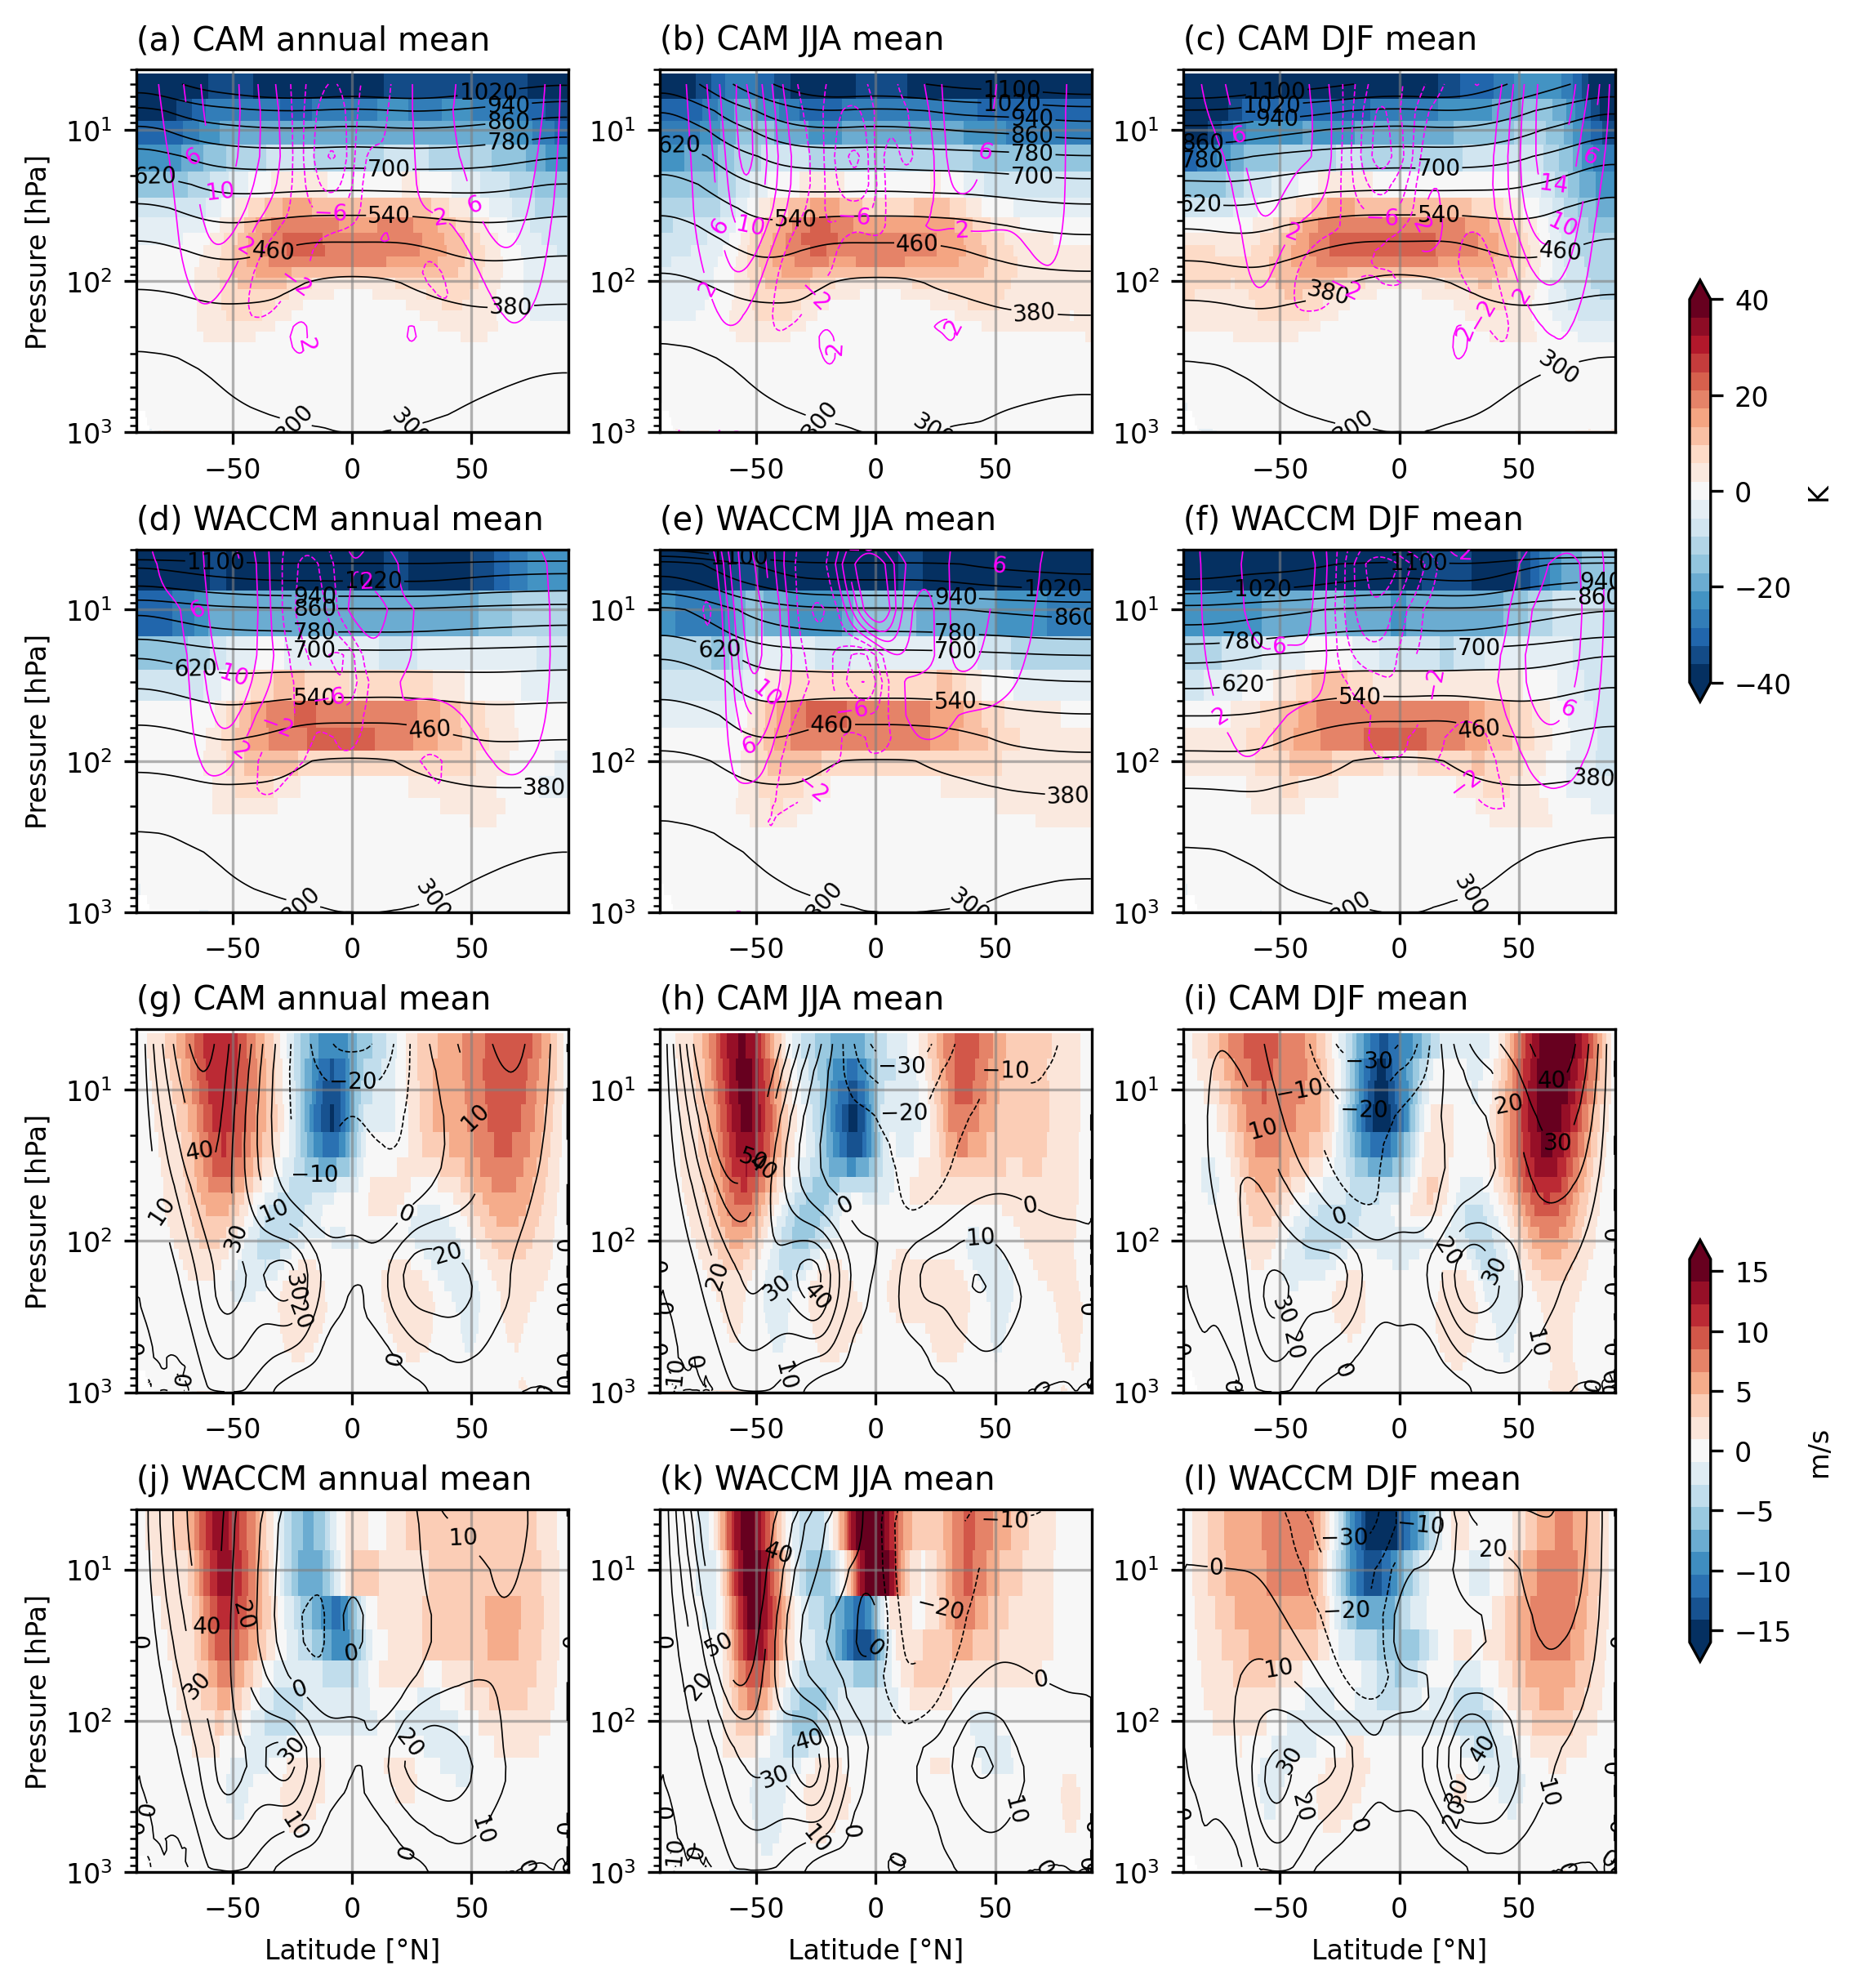
\includegraphics[width=0.95\linewidth]{images/th_U_full.png}
	\caption{(a-f): Zonal mean potential temperature anomaly of SAI 2020 compared to Reference for (a-c) CAM and (d-f) WACCM, annual, JJA and DJF mean shown for both models. Reference potential temperature shown in magenta contours, zonal mean zonal wind anomalies shown in black contours; (g-l): Zonal mean zonal wind anomaly of SAI 2020 compared to Reference for WACCM and CAM analogous to (a-f), Reference zonal wind shown in black contours.}
	\label{fig:th_U_full}
\end{figure}